\documentclass[./00PhotoBox.tex]{subfiles}
\graphicspath{{\subfix{./img/}}}
\begin{document}
\renewcommand{\itemautorefname}{Anforderung}

\chapter{Software-Entwicklung}
\label{c:software}

Für die Steuerung der Kameras und die anschließende Berechnung des 3D-Modelles muss eine Steuerungssoftware für das Kamerasystem und eine entsprechende Schnittstelle zu einer \Gls{SfM}-Software geschaffen werden. Die Entwicklung erfolgte hauptsächlich in Python in Form von Prototyping. Dieses Kapitel beschreibt die Anforderungen an die Software (siehe \autoref{sec:Anforderungsanalyse}) und die zu implementierenden Anwendungsfälle (siehe \autoref{sec:Anwendungsfallmodellierung}). Abschließend wird die Implementation (siehe \autoref{sec:Implementierung}) erarbeitet.

\section{Anforderungsanalyse}
\label{sec:Anforderungsanalyse}

Die notwendigen Anforderungen an das System wurden aus \autoref{c:einleitung} und \ref{c:photogrammetrie} abgeleitet und in diesen Abschnitt in Form von Anwendungsfällen und eines Lastenheftes aufgezeichnet. Sie wurden in funktionale und nicht-funktionale Anforderungen unterteilt. Die funktionalen Anforderungen beschreiben, was das System leisten soll, die nicht-funktionalen Anforderungen beschreiben, wie das System arbeiten soll. \todo{Quelle Fernuni Hagen?}


\subsection{Anwendungsfallmodellierung}
\label{sec:Anwendungsfallmodellierung}

Entsprechend der benötigten Schritte aus \autoref{c:photogrammetrie} und \autoref{img:ablauf} wurden die Anwendungsfälle, die die Benutzeroberfläche ermöglichen soll, im Anwendungsfall-Dia\-gramm in \autoref{img:anwendungsfall} zusammengetragen. Entsprechend der Anforderung einer einfach gehaltenen Bedienung des Systems, ist die Anzahl der verschiedenen Anwendungsfälle gering. Hauptanwendungsfall ist die Erzeugung eines 3D-Modelles, welches in mehrere Unterfälle unterteilt ist, je nach verwendeter \Gls{SfM}-Software. Es soll aber auch möglich sein, Teilschritte dieser Anwendungsfälle wie das Aufnehmen der Bilder, das Identifizieren der Passpunkte oder das Verbinden der Kameras manuell auszulösen.

\begin{figure}
    \centering
    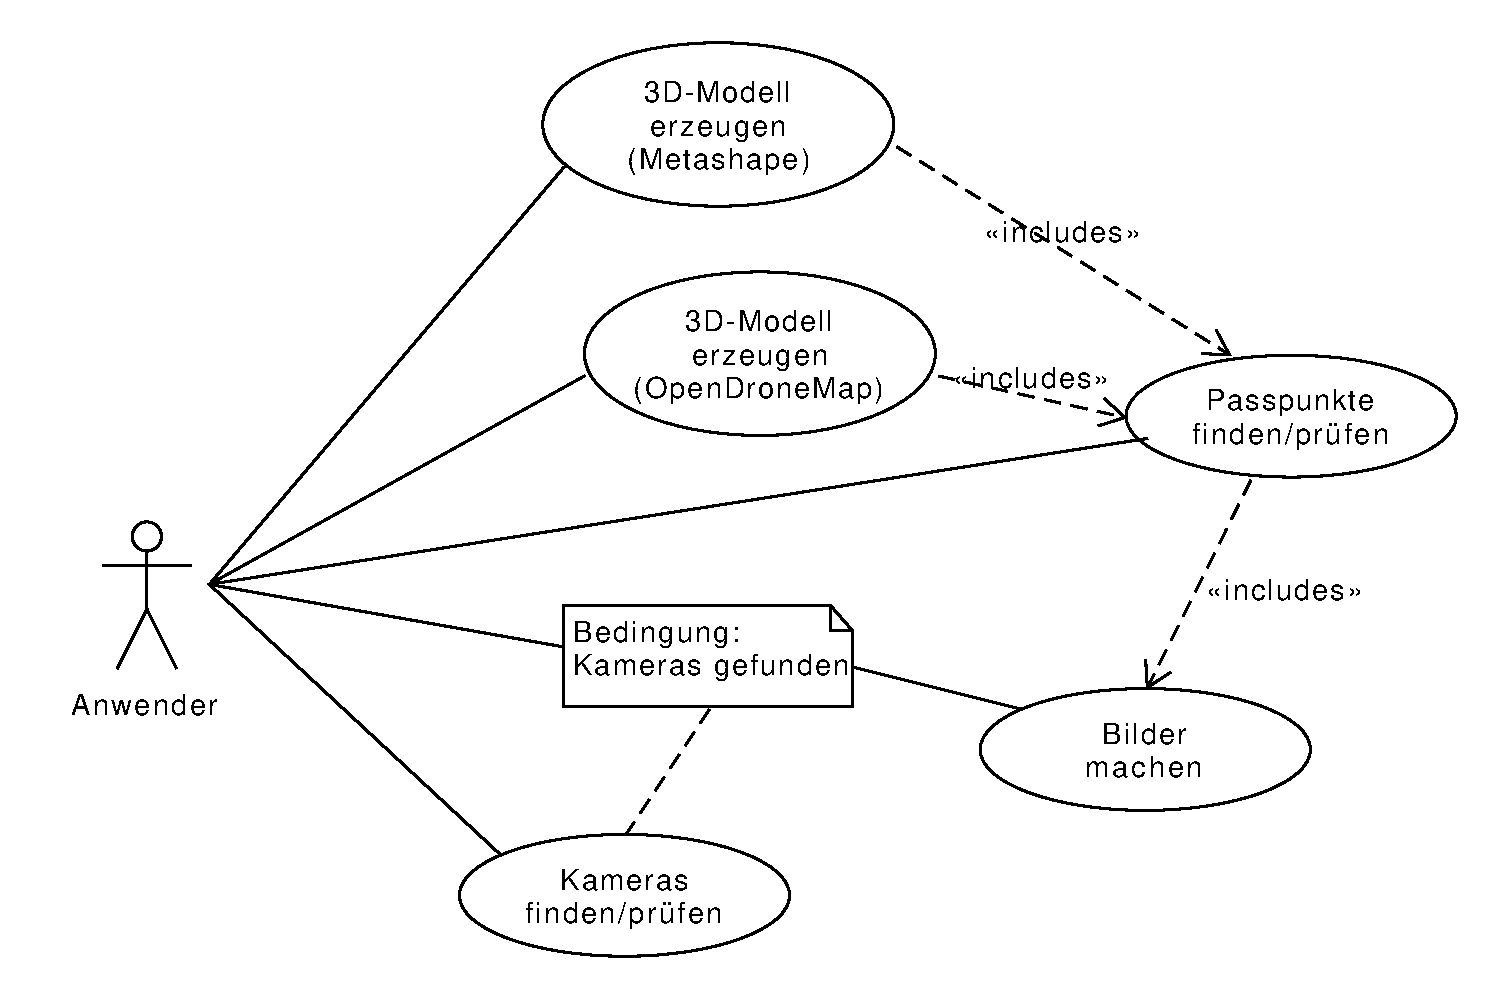
\includegraphics[width=1\textwidth]{./img/uml/uml_usecases.pdf}
    \caption{Anwendungsfall-Diagramm}
    \label{img:anwendungsfall}
\end{figure}


\subsection{Funktionale Anforderungen}
\begin{enumerate}[label=F\arabic*]
    \item \label{e:zeitgleich} Die Kameras sollen zeitgleich auslösbar sein. Es soll möglichst ver\-zögerungs\-frei ausgelöst werden.
    \item \label{e:button} Die Steuerung soll unabhängig von anderen Geräten möglich sein, beispielsweise per Tastensteuerung.
    \item \label{e:status} Der Status des Systems soll für den Nutzer erkennbar sein - auch ohne Anschluss eines Computers.
    \item \label{e:passpunkte} Es sollen Passpunkte automatisch gefunden und für die Bestimmung der äußeren Orientierung genutzt werden.
    \item \label{e:scharf} Die Bilder sollen scharf und fokussiert sein.
    \item \label{e:licht} Die Belichtung soll automatisch erfolgen, jedoch die Helligkeit der Bilder identisch sein.
\end{enumerate}

\subsection{Schnittstellen}

\begin{enumerate}[label=S\arabic*]
    \item \label{e:intspeicher} Die Daten sollen intern gespeichert werden.
    \item \label{e:usbspeicher} Eine Speicherung auf tragbaren Speichermedien wie USB-Sticks soll möglich sein.
    \item \label{e:sfmsoftware} Eine direkte Übertragung an \Gls{SfM}-Software soll möglich sein.
\end{enumerate}

\subsection{Nicht-funktionale Anforderungen}
\begin{enumerate}[label=N\arabic*]
    \item \label{e:standalone} Die Erfassung soll ohne weitere Hardware möglich sein. Das System soll unabhängig von Netzwerkanschlüssen etc. sein.
    \item \label{e:wlan} Jegliche Kommunikation soll über WLAN erfolgen.
\end{enumerate}


\section{Anwendungsentwurf}
Der Anwendungsentwurf legt die grundlegenden Strukturen der Software fest. Hierbei wird festgelegt, welche Module benötigt werden und wie diese miteinander kommunizieren. Diese Struktur wird einmalig festgelegt und bildet die Grundlage für die Implementierung.

\subsection{Domänen-Klassendiagramm}
Aus den für die Berechnungen des 3D-Modelles benötigten Daten wurde das Domänen-Klassendiagramm aus \autoref{img:dokladia} erzeugt. Dieses zeigt vor allem die Abhängigkeiten der einzelnen Datensätze untereinander. Es bildet hiermit die Grundlage für die Datenschnittstellen der einzelnen Komponenten zueinander und den jeweils benötigten Datensätzen.

Zur Berechnung eines 3D-Modells werden die inneren und äußeren Orientierungen der Kameras benötigt (vgl. \autoref{c:photogrammetrie}). Da die \gls{innereOrientierung} der Kameras instabil ist, reichen hier Näherungswerte. Entsprechend wurde diese nicht wie üblich pro Kamera, sondern nur pro Modell festgehalten. Die Klasse \textit{CameraModel} hat daher neben dem Namen Attribute für die Parameter der inneren Orientierung in Form einer Geradengleichung abhängig von der Fokussierung. Jede Kamera hat dann (pro Messung) eine Position  \textit{Point3D} und drei Drehwinkel, hierdurch wird die \gls{aeussereOrientierung} im Modell abgebildet. Um die Passpunktpositionen festzuhalten, wird das Objekt \textit{PasspointPosition} verwendet. Dieses speichert die Position des Passpunktes in den Bildern der Kameras als \textit{Point2D} und die Position im Raum als \textit{Passpoint}. Außerdem verweist die Klasse auf das entsprechende Bild \textit{Image}, welches wiederum auf die Kamera \textit{Camera} verweist. Die Klasse \textit{Image} hält des Weiteren die Attribute für den Dateinamen und die genutzte Fokussierung.

\begin{figure}
    \centering
    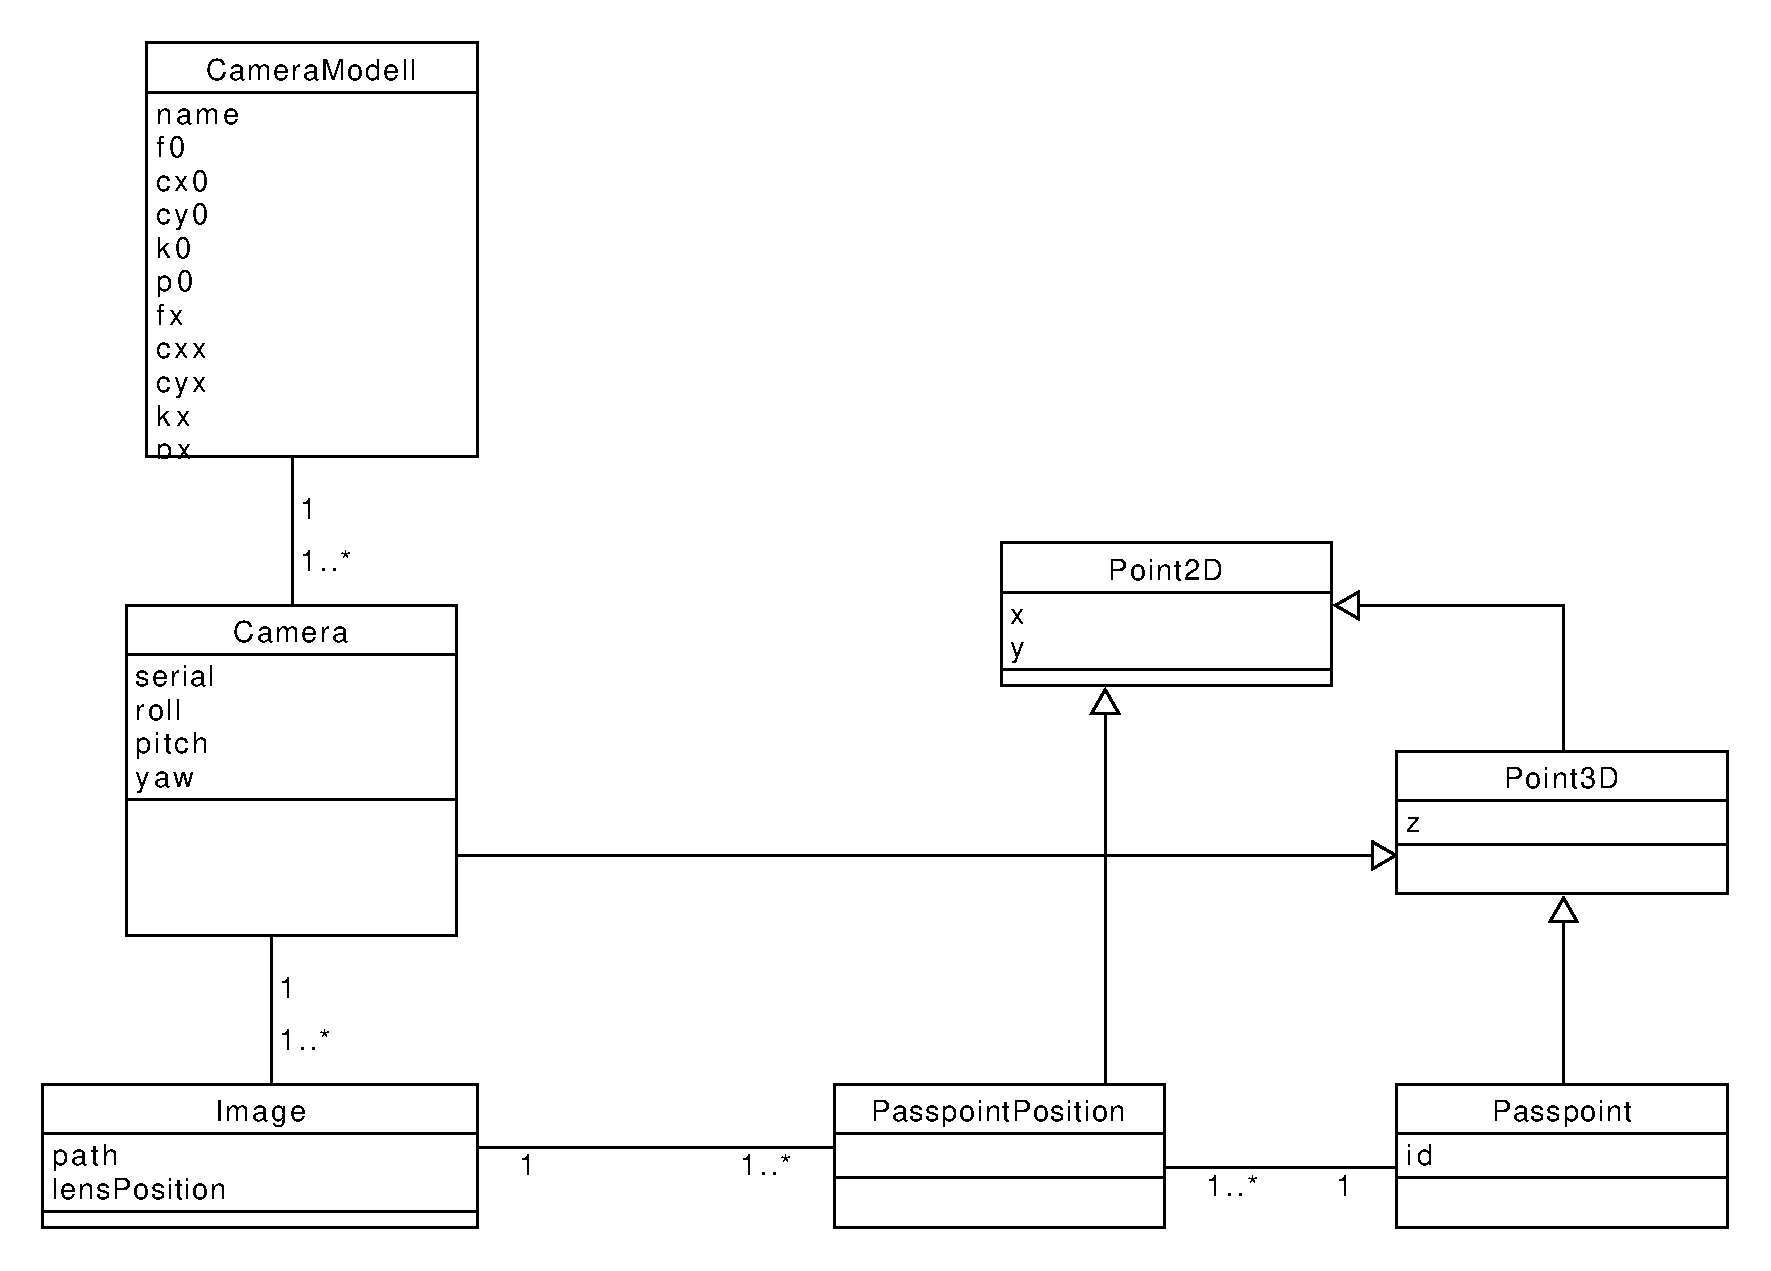
\includegraphics[width=1\textwidth]{./img/uml/uml_domain.pdf}
    \caption{Domänen-Klassendiagramm}
    \label{img:dokladia}
\end{figure}

\subsection{Programmablauf}
Die Kommunikation innerhalb des Systems ist in dem Ablaufdiagramm in \autoref{img:uml_sequence_capture} dargestellt. Eine Auslösung der Kamera erfolgt über den Software-Button in der Desktop-Software, dem Webinterface oder über einen Taster. Optional werden die Belichtungen der Kameras synchronisiert und anschließend die Aufnahmen erzeugt. Die Raspberry Pi Zero W senden die Aufnahmen und die gefundenen ArUco-Marker an den Raspberry Pi 4. Dieser berechnet die Kamerapositionen und speichert die Daten. Die Desktop-Software kann die Daten dann herunterladen und an die \Gls{SfM}-Software übergeben, welche ein 3D-Modell erzeugt. Auf die Details der einzelnen Module wird in \autoref{sec:Implementierung} eingegangen.


\begin{figure}
    \centering
    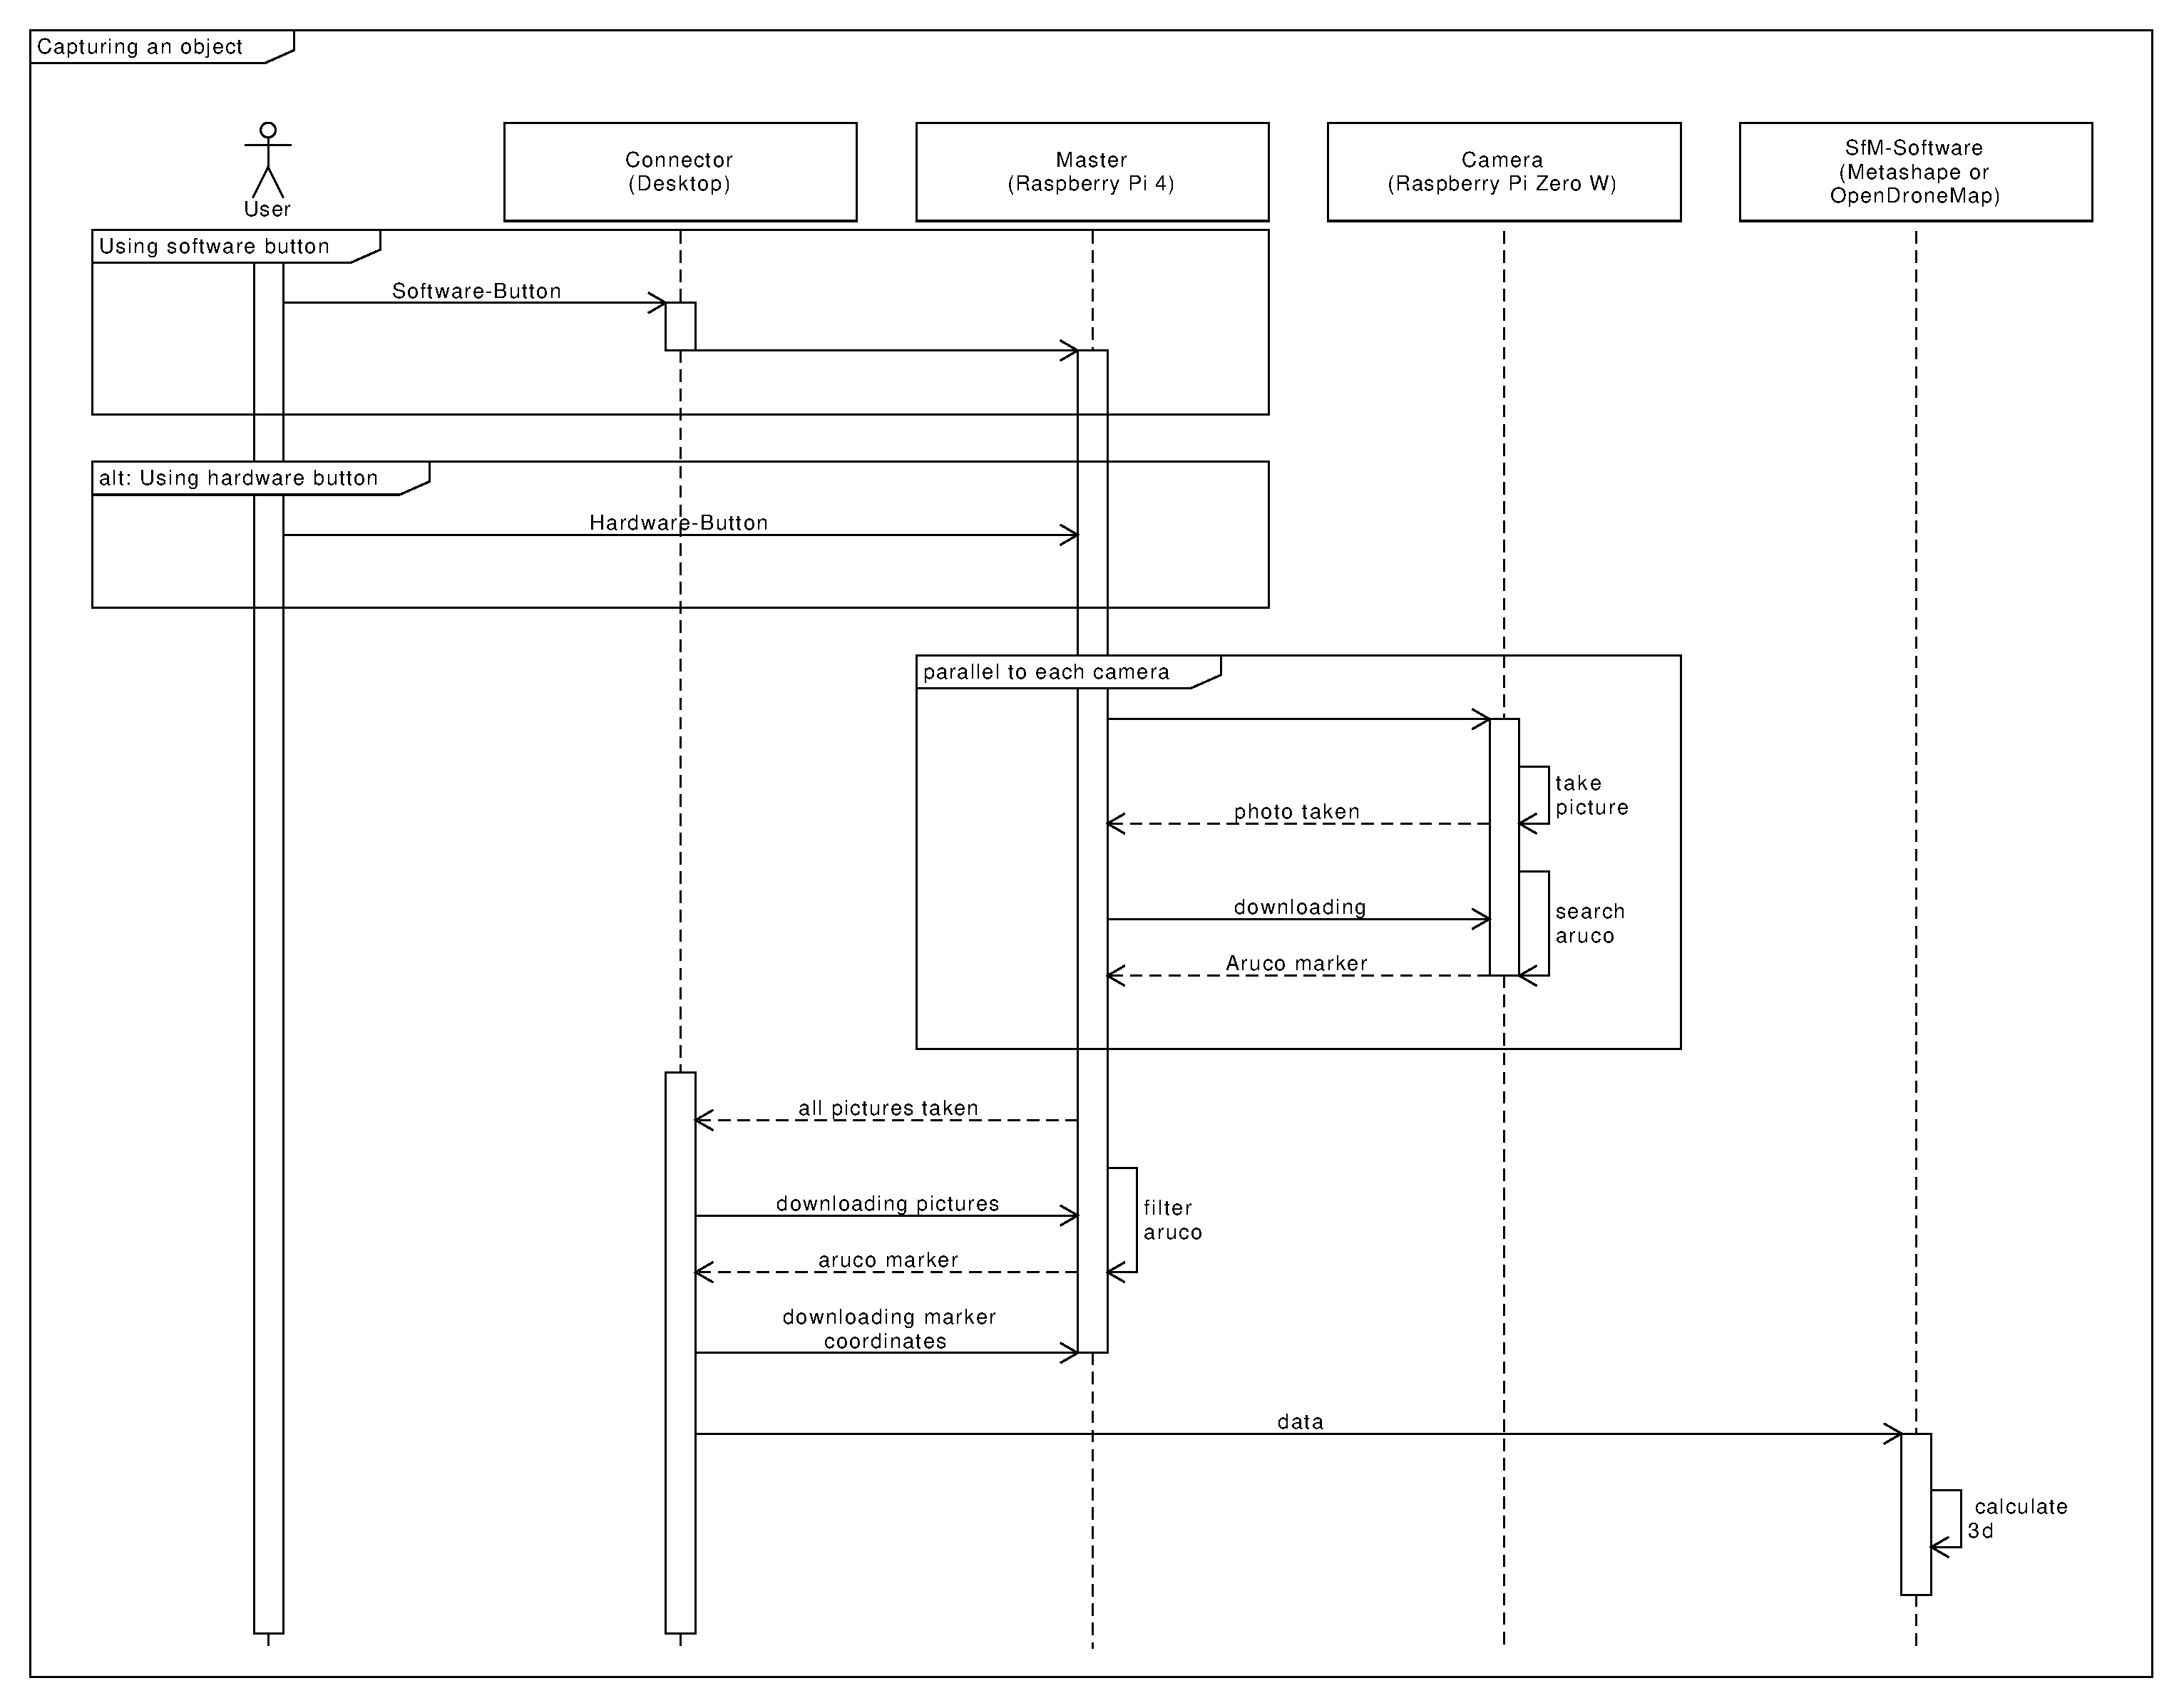
\includegraphics[width=1\textwidth]{./img/uml/uml_sequence_capture.pdf}
    \caption{Ablaufdiagramm zur Kommunikation bei der Aufnahme eines 3D-Modelles}
    \label{img:uml_sequence_capture}
\end{figure}


\section{Implementierung}
\label{sec:Implementierung}

Die Programmierung des Systems erfolgte iterativ. Einzelne Arbeitspakete wurden in einem Jupyter-Notebook ausprobiert und dann, wenn dieser Schritt erfolgreich war, in den Gesamtworkflow integriert - teilweise sind diese im \autoref{c:voruntersuchungen} beschrieben. Größtenteils wurde der Python-Code objektorientiert und typisiert geschrieben. Die Teile, die auf einem Desktoprechner ausgeführt werden sollen, wurden in Java geschrieben, da hier später die Einrichtung auf verschiedenen Rechnern und Plattformen einfacher ist.


\subsection{Module auf den Raspberry Pi (Python)}
Die Software auf den Raspberry Pi wurde in Python geschrieben. Hierbei wurde darauf geachtet, dass die Module möglichst unabhängig voneinander sind und nur über definierte Schnittstellen kommunizieren.

\subsubsection{Bibliotheken}
Es wurde, wenn möglich, auf fertige Python-Bibliotheken zurückgegriffen. Hierdurch sollte der Programmieraufwand verringert und auf bereits getesteten Code gesetzt werden. Außerdem greifen viele der Bibliotheken wie OpenCV oder NumPy auf hardwarenahe Berechnungen zurück, sodass der Geschwindigkeitsnachteil von Python nicht weiter ins Gewicht fällt. Die wichtigsten Bibliotheken sind:

\paragraph{OpenCV}
ist eine Bibliothek für Bildbearbeitung und maschinelles Sehen. Sie ist weit verbreitet und bietet viele photogrammetrische Funktionen. Hiermit wurde beispielsweise die Detektion von Markern durchgeführt und die Näherungswerte der Kameras berechnet.

\paragraph{SciPy}
stellt Methoden für wissenschaftliche Berechnungen bereit, beispielsweise für verschiedene Formen von Ausgleichungsrechnungen. Sie wurde für die Berechnung der Bündelblockausgleichung verwendet. Der manuelle Ansatz mit Formeln aus \cite{luhmann} unter Nutzung von nur von NumPy war sehr ressourcenlastig. Mit Unterstützung von SciPy und der Projektionsgleichung konnte die Berechnungsdauer stark dezimiert werden.

\paragraph{NumPy}
bietet Datenstrukturen für Matrizen und Vektoren sowie effiziente Berechnungen mit diesen. Sie wurde beispielsweise für die Berechnung der Kamerapositionen und die Bündelblockausgleichung genutzt, ist aber auch Grundlage für OpenCV und SciPy.


\paragraph{Flask}
ist ein Webframework für Python. Es wurde genutzt um die Weboberfläche und die Datendownloads bereitzustellen. Hiermit wurde ein Webserver aufgesetzt, der die Daten der Kameras anzeigt und die Steuerung ermöglicht.

\paragraph{rpi-ws281x}
\label{p:ws281x}
ermöglicht die Steuerung der RGB-LEDs. Hierzu wird das in \cite{ws2811} beschriebene Steuerprotokoll von der Bibliothek implementiert. Die Steuerung kann dann mittels einfacher Farbcodes erfolgen.

\subsubsection{Allgemeine Module}
In \autoref{img:uml_common} werden Klassen dargestellt, die in allen Modulen genutzt werden. Diese sind verantwortlich für allgemeine Funktionen wie das Logging und das Auslesen der Konfiguration. Die Klasse \texttt{Config} liest die Konfiguration aus einer Datei aus und stellt diese zur Verfügung. \texttt{Logger} ermöglicht das Loggen von Informationen und Fehlern in einer Textdatei, in den Systemprotokollen und/oder die Ausgabe auf dem Terminal bei manuellem Start. Die Klassen \texttt{CamSettings} und \texttt{ArucoMarkerPos} sind Datenklassen, die die Einstellungen der Kameras und die Position der ArUco-Marker speichern. Diese Daten werden zwischen der Master-Steuerung und der Kamera-Steuerung ausgetauscht -- hierdurch wird sichergestellt, dass das erwartete Datenmodell auf beiden Seiten gleich ist. \texttt{CamSettings} werden dabei vom Raspberry Pi 4 an die Raspberry Pi Zero W gesendet, um die Kameras zu konfigurieren. \texttt{ArucoMarkerPos} werden von den Raspberry Pi Zero W an den Raspberry Pi 4 gesendet, um die Position der identifizierten ArUco-Marker zu übertragen.

\begin{figure}
    \centering
    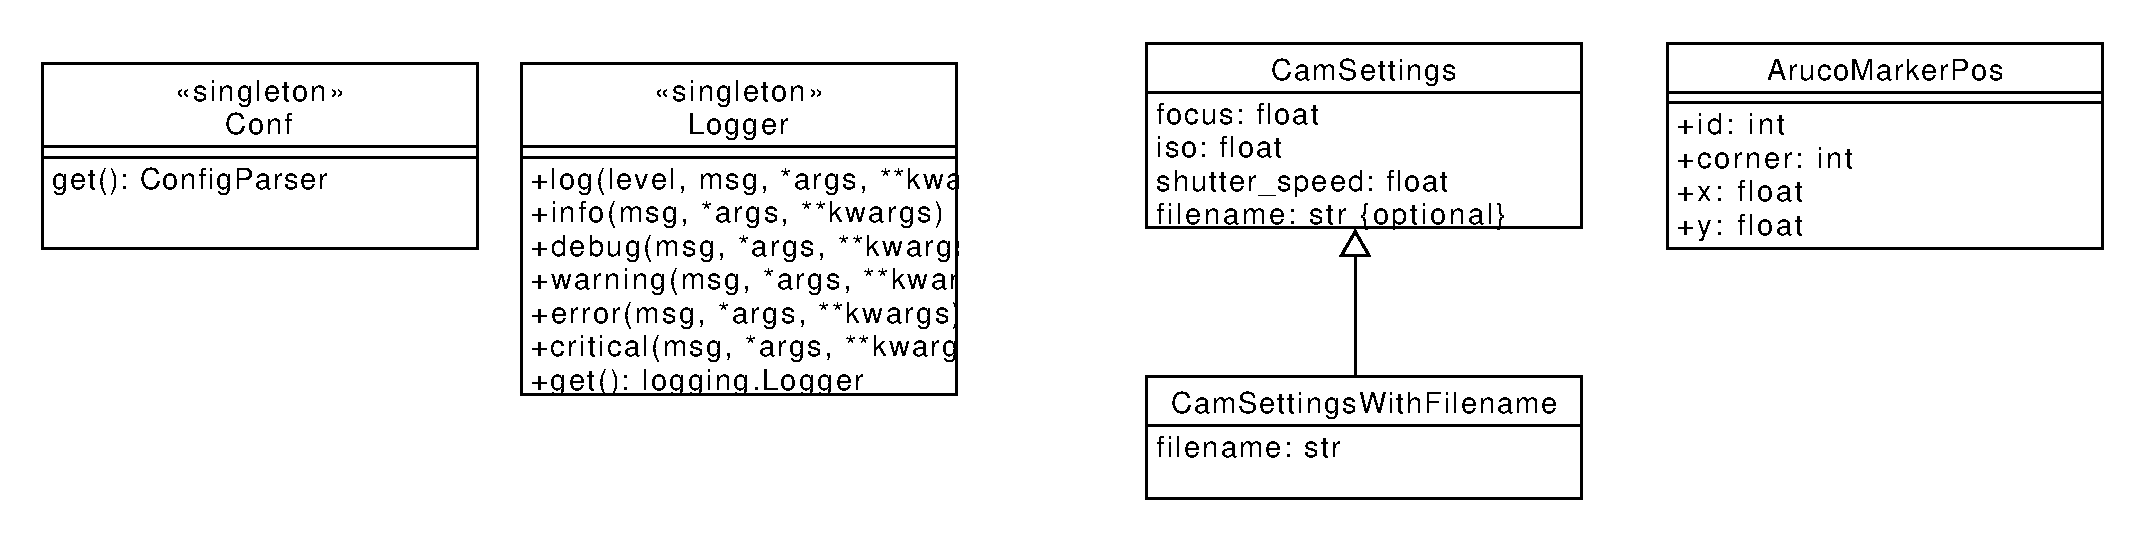
\includegraphics[width=1\textwidth]{./img/uml/uml_common_classdiagramm.pdf}
    \caption{Klassen des Common-Package}
    \label{img:uml_common}
\end{figure}


\subsubsection{Master-Steuerung}

Auf einem Raspberry Pi 4 läuft die Gesamt\-steuerung des Systems. Dieses stellt Schnitt\-stellen zur Steuerung auf drei verschiedenen Wegen bereit: per Taster, per Weboberfläche und per \Gls{Socket}-Verbindung. Außerdem stellt es die Daten per \Gls{REST}-Schnittstelle zur Verfügung. Die Klassen sind in \autoref{img:master} dargestellt.

Das Skript \texttt{Master} wird automatisch bei Systemstart über \texttt{systemd} als Daemon -- als im Hintergrund und dauerhaft laufender Service \citep[S. 369]{negus2020linux} -- gestartet. Hier ist die Webschnittstelle implementiert. Sie ermöglicht die komplette Steuerung, das Konfigurieren sowie das Anzeigen und Herunterladen der Bilder. Das Skript instanziiert außerdem die Klasse \texttt{Control}, welche die hauptsächliche Steuerung übernimmt und den Kern des Systems darstellt.

Die Steuerung per Taster implementiert die Klasse \texttt{ButtonControl}. Sie ermöglicht einfache Aufgaben wie das Suchen von Kameras, das Aufnehmen von Bilder und die Aktivierung des Standbys bzw. das Herunterfahren des Systems auch ohne PC durchzuführen (\autoref{e:button}). Die Klasse \texttt{DesktopControlThread} startet, wie der Name bereits vermuten lässt, als eigenständiger Thread und stellt eine \Gls{Socket}-Verbindung zur Kommunikation mit der Desktop-Software und die Steuerung hierüber bereit. Einen weiteren Thread stellt \texttt{CameraControlThread} zur Verfügung. Dieser überwacht das Netzwerk auf Nachrichten der Kameras und initiiert die entsprechenden Schritte. Die eigentlichen Verarbeitungsschritte werden in der Klasse \texttt{Control} durchgeführt. Auch für diese Aufgaben werden zum Teil eigene Threads gestartet, damit die Verarbeitung parallel erfolgen kann. Beispielsweise wird der Download der Bilder und die Berechnung von Kamerapositionen in eigenen Threads durchgeführt.

Die \texttt{Control}-Klasse steuert die Aufnahme, sammelt die Daten der einzelnen Kameras und stellt diese zur Weiterverarbeitung zur Verfügung. Sie sendet eingehende Aufträge als Broadcast-Nachrichten in das Netzwerk an die Raspberry Pi Zero W mit den Kameras, die dann beispielsweise Bilder aufnehmen. Hierdurch wird die nahezu zeitgleiche Auslösung gewährleistet (\autoref{e:zeitgleich}), die bei einer einzelnen Ansteuerung als Schleife nicht möglich wäre. Zur Vereinheitlichung der Belichtung kann eine Funktion aktiviert werden, sodass erst einmal die Belichtung von jeder Kamera berechnet und diese dann von der \texttt{Control}-Klasse gemittelt wird. Dadurch werden dann alle Bilder mit der gleichen Einstellung aufgenommen, sodass keine Helligkeitsunterschiede zwischen den Aufnahmen bestehen (\autoref{e:licht}).
Nach der Aufnahme der Bilder und der Erkennung der ArUco-Marker werden die Daten von den Raspberry Pi Zero W an den Raspberry Pi 4 übertragen. Aus den ArUco-Markern wird die \gls{aeussereOrientierung} der Kameras als Näherungswerte bestimmt (\autoref{e:passpunkte}). Die Daten werden anschließend in einem Archiv gespeichert (\autoref{e:intspeicher}).

Die Datenübertragung an die Desktop-Software erfolgt über die \Gls{REST}-Schnittstelle, die wieder vom \texttt{Master}-Skript bereitgestellt wird. Alternativ kann auch ein USB-Stick an dem Raspberry Pi angesteckt werden (\autoref{e:usbspeicher}) oder die Daten über die Weboberfläche manuell heruntergeladen werden. Dazu wird bei der Verarbeitung der Daten geprüft, ob ein USB-Stick angeschlossen ist. Falls dieses der Fall ist, wird dieser gemountet, die Daten kopiert und der Stick wieder ausgehängt, damit dieser (fast) jederzeit getrennt werden kann. Das Datenformat auf dem USB-Stick und in den Archiv-Dateien aus der Weboberfläche entspricht dem, welches die Desktop-Software anlegt. So kann diese die Daten dann auch einladen und weiterverarbeiten.

\begin{figure}
    \centering
    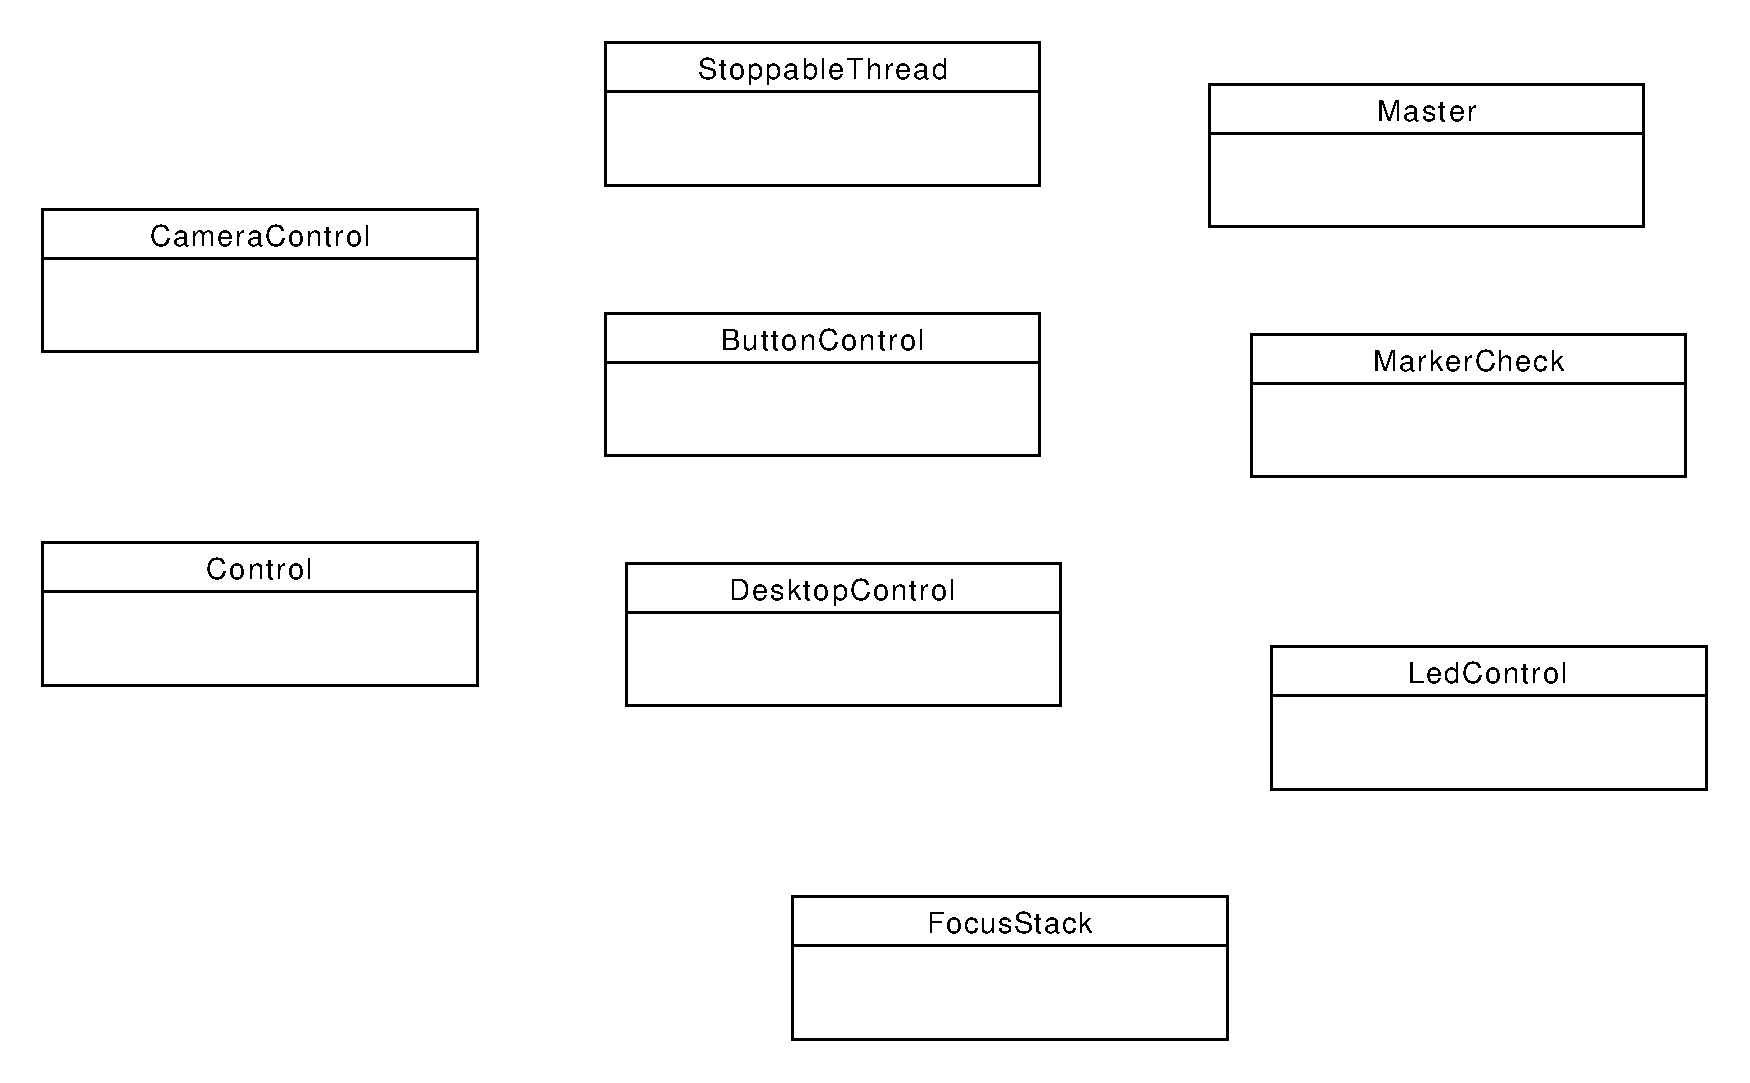
\includegraphics[width=1\textwidth]{./img/uml/uml_master_classdiagramm.pdf}
    \caption{Klassen des Master-Package}
    \label{img:master}
\end{figure}


\subsubsection{Kamera-Steuerung}
Die Raspberry Pi Zero W übernehmen die Steuerung der Kameras. Hierfür wurde ein Modul entwickelt, dass die Kameras steuert, die Bilder aufnimmt und anschließend dem steuernden Raspberry zur Verfügung stellt. Die Klassen sind in \autoref{img:uml_camera} dargestellt.

Das Skript \texttt{Camera} wird automatisch bei Systemstart über \texttt{systemd} als Daemon gestartet. Es erzeugt dann über Flask eine einfache Weboberfläche, über die die Kameras konfiguriert und die Bilder betrachtet werden können. Außerdem stellt das Skript auch die \Gls{REST}-Schnittstelle bereit, über das die Bilder und gefundenen Passpunkte abgerufen werden können. Die Klasse \texttt{CameraControl} wird vom Skript instanziiert und übernimmt die eigentliche Steuerung. Sie nimmt die Konfiguration entgegen und setzt diese um. Sie überwacht das Netzwerk auf Broadcast-Nachrichten der Master-Steuerung und initiiert die entsprechenden Schritte.  Über die gleiche \Gls{Socket}-Verbindung meldet sie auch den Status an die Master-Steuerung, beispielsweise wenn Bilder aufgenommen wurden oder die Erkennung der Passpunkte abgeschlossen ist. Die Klasse \texttt{CameraInterface} wird von \texttt{CameraControl} aufgerufen, bildet ein Adapter für das Kameramodul und kapselt so die Hardwaresteuerung. Sie nimmt die Bilder auf und speichert diese. Gegebenenfalls leitet sie die Bilder an \texttt{CameraAruco}-Klasse weiter, damit diese in einem eigenen Thread die ArUco-Marker identifizieren kann (\autoref{e:passpunkte}).

\begin{figure}
    \centering
    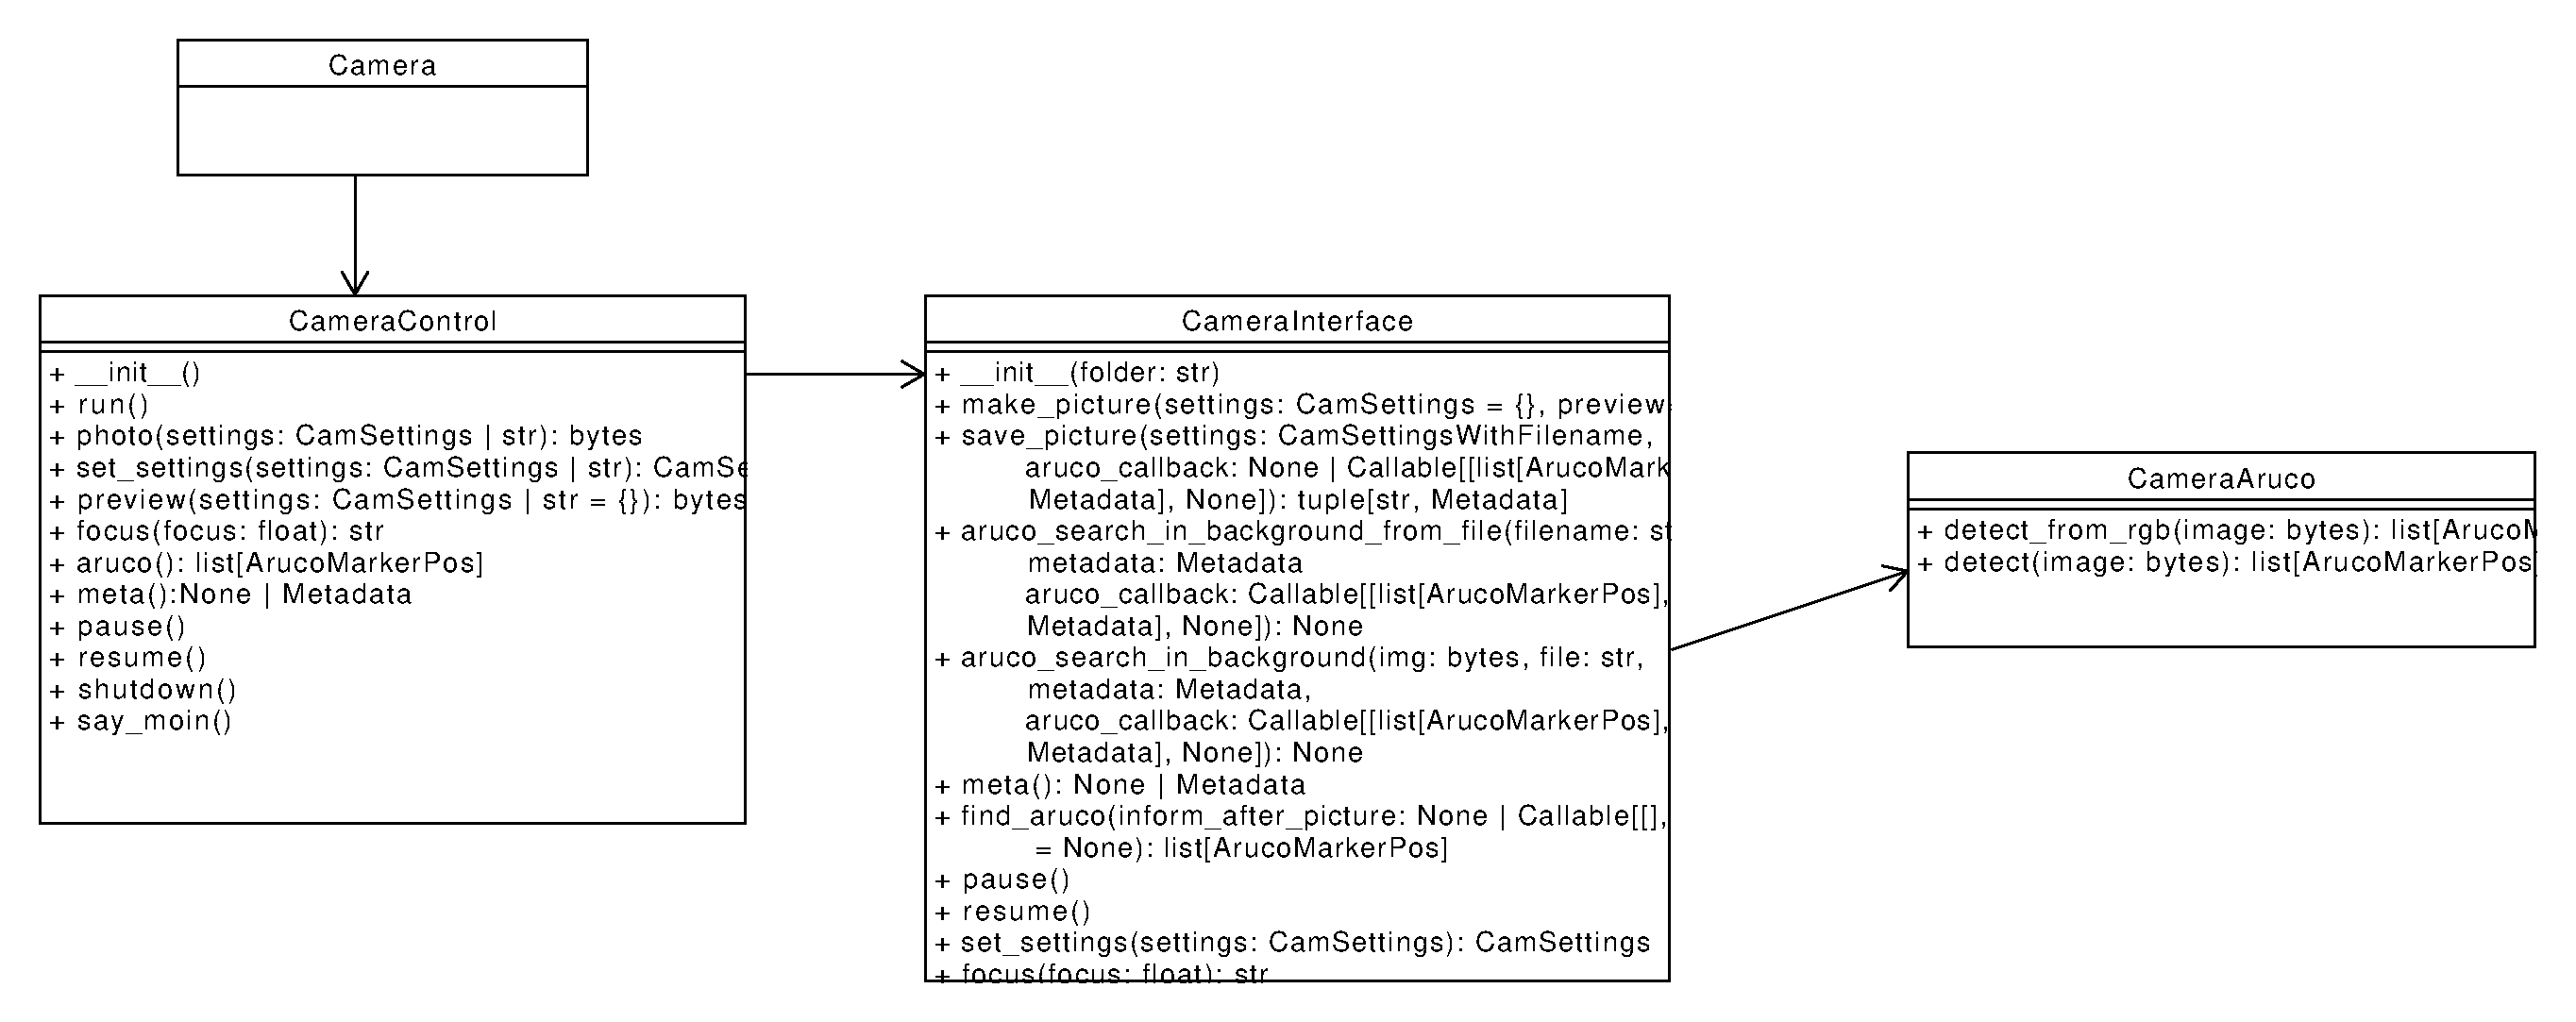
\includegraphics[width=1\textwidth]{./img/uml/uml_camera_classdiagramm.pdf}
    \caption{Klassen des Camera-Package}
    \label{img:uml_camera}
\end{figure}


\subsection{Desktop-Schnittstelle (Java)}
Die Desktop-Schnittstelle dient zur Steuerung des Systems und zur automatischen Über\-tragung der Daten an die \Gls{SfM}-Software (\autoref{e:sfmsoftware}). Sie wurde in Java geschrieben, um eine einfache Nutzung auf verschiedenen Betriebssystemen zu ermöglichen. Die \Gls{API} für Java der \Gls{SfM}-Software Agisoft Metashape kann im Gegensatz zur Python-\Gls{API} ohne Installation verwendet werden. Die Software kommuniziert mit dem Raspberry Pi 4 hauptsächlich über eine \Gls{Socket}-Verbindung, wobei jedoch die Datenübertragung der Bilder vom Raspberry Pi 4 zur Desktop-Software über die \Gls{REST}-Schnittstelle erfolgt. Neben der Übertragung der Bilder an die \Gls{SfM}-Software ermöglicht die Software das Starten von Aufnahmen. Ein Screenshot der Benutzeroberfläche ist in \autoref{img:screenshot_connector} dargestellt. Die Schnittstellen-Software unterstützt als \Gls{SfM}-Software aktuell Agisoft Metashape und OpenDroneMap, jedoch ist die Schnittstelle so gestaltet, dass auch andere Software ergänzt werden könnte.

Die Klassen sind in \autoref{img:uml_connector} dargestellt. \texttt{Connector} stellt hierbei den Einstiegspunkt dar. Die Klasse instanziiert die Benutzeroberfläche \texttt{ConnectorGui} und übernimmt die Steuerung der Software. Die Klasse \texttt{PhotoBoxClient} wird beim Klick auf Verbinden von \texttt{Connector} gestartet und übernimmt die Kommunikation mit dem Raspberry Pi 4. Sie sendet die Steuerbefehle und empfängt die Daten. Außerdem wird eine Klasse, die das Interface \texttt{SfmClient} implementiert aufgerufen. Diese Klasse stellt die Schnittstelle zur \Gls{SfM}-Software dar. Hierbei wird je nach Auswahl der Software \texttt{MetashapeClient}, \texttt{OpenDroneMapClient} oder \texttt{DownloadClient} instanziiert. Diese Klasse übernimmt die Kommunikation mit der entsprechenden \Gls{SfM}-Software und übergibt die Daten. \texttt{DownloadClient} stellt einen Sonderfall dar, hier werden die Daten nur gespeichert, um sie später weiterverarbeiten zu können.

\begin{figure}
    \centering
    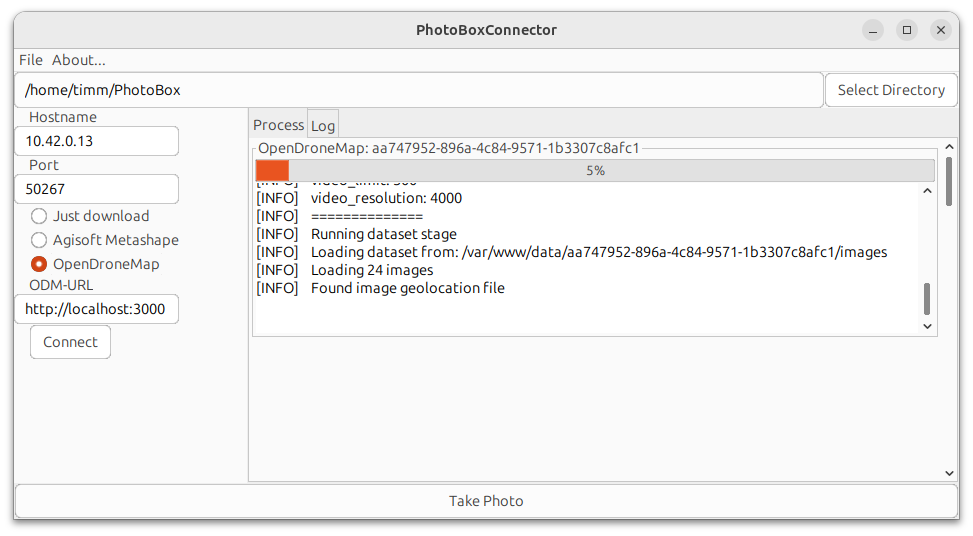
\includegraphics[width=1\textwidth]{./img/5_software/connector_screenshot.png}
    \caption{Screenshot der Connector-Software unter Ubuntu 24.04}
    \label{img:screenshot_connector}
\end{figure}

\begin{figure}
    \centering
    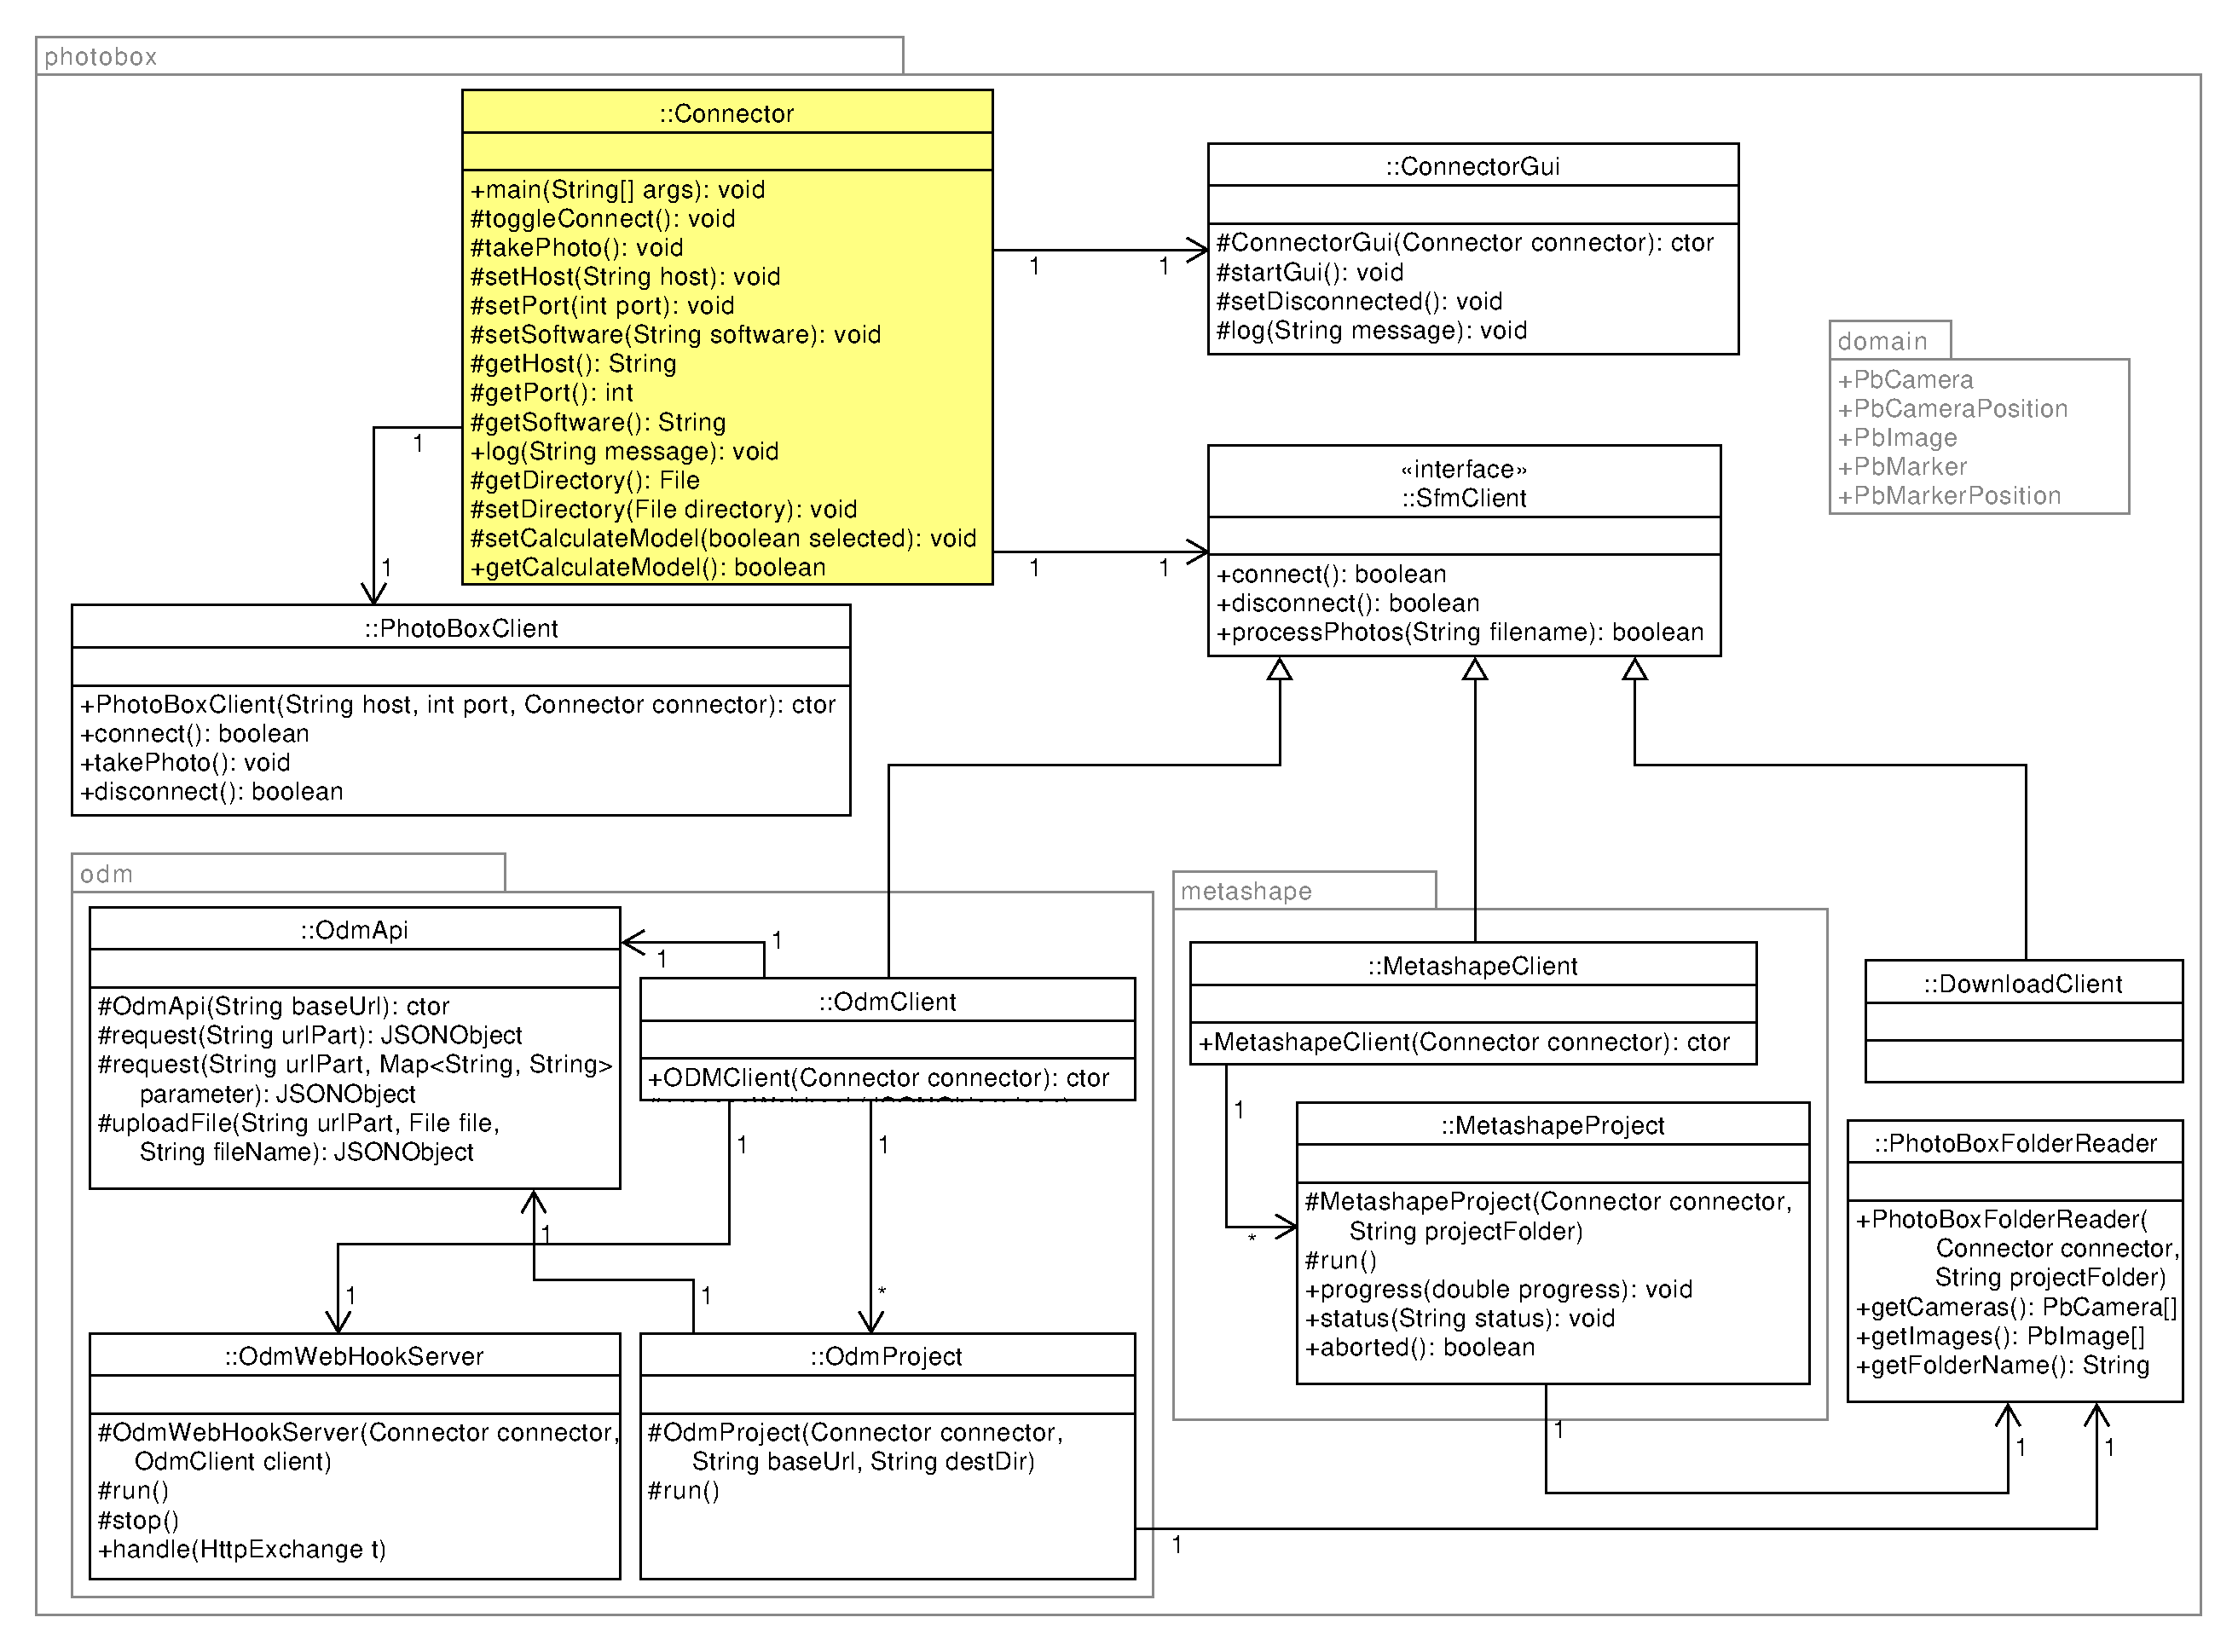
\includegraphics[width=1\textwidth]{./img/uml/uml_connector_classdiagramm.pdf}
    \caption{Connector-Package}
    \label{img:uml_connector}
\end{figure}

\subsection{Konfiguration}
Neben der eigentlichen Programmierung erfolgten noch verschiedene Konfigurationen, um das System zu betreiben. Diese sollen hier kurz vorgestellt werden.

\paragraph{WLAN-Router}
Der WLAN-Router wurde so konfiguriert, dass er ein WPA2-ver\-schlüssel\-tes WLAN-Netzwerk aussendet. Außerdem wurde er als DHCP-Server eingerichtet, der den angeschlossenen Geräten automatisch eine IP-Adresse zuweist. Die IP-Adressen der Raspberry Pi wurden fest vergeben, um die Kommunikation zu erleichtern. Der Router wurde so konfiguriert, dass er die Kommunikation zwischen den Raspberry Pi einem per Kabel angeschlossenen Desktop-PC zulässt, aber auch eine per Netzwerk-Kabel angeschlossene Internetverbindung durchleitet.

\paragraph{Raspberry Pi 4}
Der Raspberry Pi 4 wurde so konfiguriert, dass er automatisch das Skript \texttt{Master} startet. Hierzu wurde ein \texttt{systemd}-Service erstellt, der das Skript beim Systemstart ausführt. Vorher wird bei Vorliegen einer Internetverbindung geprüft, ob das Git-Repository eine neue Version der Software zur Verfügung stellt. Falls dieses der Fall ist, wird dieses heruntergeladen und installiert.

Zur Beschleunigung von Softwareupdates des Betriebssystems, wurde ein entsprechender apt-Proxyservice eingerichtet. Dieser speichert die heruntergeladenen Pakete und stellt diese bei Bedarf den Raspberry Pi Zero W zur Verfügung. Hierdurch wird die Bandbreite des Internetanschlusses geschont und die Updates können schneller durchgeführt werden.

\paragraph{Raspberry Pi Zero W}
Die Raspberry Pi Zero W wurden so konfiguriert, dass sie automatisch das Skript \texttt{Camera} starten. Hierzu wurde ebenfalls ein \texttt{systemd}-Service erstellt, der das Skript beim Systemstart ausführt. Auch hier wurde der bereits beschriebene Update-Mechanismus eingebaut. Entsprechend der Cache-Konfiguration des Raspberry Pi 4 wurde hier der apt-Proxyservice als Paketquelle eingerichtet.


\biblio
\end{document}